% Options for packages loaded elsewhere
\PassOptionsToPackage{unicode}{hyperref}
\PassOptionsToPackage{hyphens}{url}
\PassOptionsToPackage{dvipsnames,svgnames,x11names}{xcolor}
%
\documentclass[
  letterpaper,
  DIV=11,
  numbers=noendperiod]{scrartcl}

\usepackage{amsmath,amssymb}
\usepackage{lmodern}
\usepackage{iftex}
\ifPDFTeX
  \usepackage[T1]{fontenc}
  \usepackage[utf8]{inputenc}
  \usepackage{textcomp} % provide euro and other symbols
\else % if luatex or xetex
  \usepackage{unicode-math}
  \defaultfontfeatures{Scale=MatchLowercase}
  \defaultfontfeatures[\rmfamily]{Ligatures=TeX,Scale=1}
\fi
% Use upquote if available, for straight quotes in verbatim environments
\IfFileExists{upquote.sty}{\usepackage{upquote}}{}
\IfFileExists{microtype.sty}{% use microtype if available
  \usepackage[]{microtype}
  \UseMicrotypeSet[protrusion]{basicmath} % disable protrusion for tt fonts
}{}
\makeatletter
\@ifundefined{KOMAClassName}{% if non-KOMA class
  \IfFileExists{parskip.sty}{%
    \usepackage{parskip}
  }{% else
    \setlength{\parindent}{0pt}
    \setlength{\parskip}{6pt plus 2pt minus 1pt}}
}{% if KOMA class
  \KOMAoptions{parskip=half}}
\makeatother
\usepackage{xcolor}
\setlength{\emergencystretch}{3em} % prevent overfull lines
\setcounter{secnumdepth}{-\maxdimen} % remove section numbering
% Make \paragraph and \subparagraph free-standing
\ifx\paragraph\undefined\else
  \let\oldparagraph\paragraph
  \renewcommand{\paragraph}[1]{\oldparagraph{#1}\mbox{}}
\fi
\ifx\subparagraph\undefined\else
  \let\oldsubparagraph\subparagraph
  \renewcommand{\subparagraph}[1]{\oldsubparagraph{#1}\mbox{}}
\fi


\providecommand{\tightlist}{%
  \setlength{\itemsep}{0pt}\setlength{\parskip}{0pt}}\usepackage{longtable,booktabs,array}
\usepackage{calc} % for calculating minipage widths
% Correct order of tables after \paragraph or \subparagraph
\usepackage{etoolbox}
\makeatletter
\patchcmd\longtable{\par}{\if@noskipsec\mbox{}\fi\par}{}{}
\makeatother
% Allow footnotes in longtable head/foot
\IfFileExists{footnotehyper.sty}{\usepackage{footnotehyper}}{\usepackage{footnote}}
\makesavenoteenv{longtable}
\usepackage{graphicx}
\makeatletter
\def\maxwidth{\ifdim\Gin@nat@width>\linewidth\linewidth\else\Gin@nat@width\fi}
\def\maxheight{\ifdim\Gin@nat@height>\textheight\textheight\else\Gin@nat@height\fi}
\makeatother
% Scale images if necessary, so that they will not overflow the page
% margins by default, and it is still possible to overwrite the defaults
% using explicit options in \includegraphics[width, height, ...]{}
\setkeys{Gin}{width=\maxwidth,height=\maxheight,keepaspectratio}
% Set default figure placement to htbp
\makeatletter
\def\fps@figure{htbp}
\makeatother
\newlength{\cslhangindent}
\setlength{\cslhangindent}{1.5em}
\newlength{\csllabelwidth}
\setlength{\csllabelwidth}{3em}
\newlength{\cslentryspacingunit} % times entry-spacing
\setlength{\cslentryspacingunit}{\parskip}
\newenvironment{CSLReferences}[2] % #1 hanging-ident, #2 entry spacing
 {% don't indent paragraphs
  \setlength{\parindent}{0pt}
  % turn on hanging indent if param 1 is 1
  \ifodd #1
  \let\oldpar\par
  \def\par{\hangindent=\cslhangindent\oldpar}
  \fi
  % set entry spacing
  \setlength{\parskip}{#2\cslentryspacingunit}
 }%
 {}
\usepackage{calc}
\newcommand{\CSLBlock}[1]{#1\hfill\break}
\newcommand{\CSLLeftMargin}[1]{\parbox[t]{\csllabelwidth}{#1}}
\newcommand{\CSLRightInline}[1]{\parbox[t]{\linewidth - \csllabelwidth}{#1}\break}
\newcommand{\CSLIndent}[1]{\hspace{\cslhangindent}#1}

\KOMAoption{captions}{tableheading}
\makeatletter
\makeatother
\makeatletter
\makeatother
\makeatletter
\@ifpackageloaded{caption}{}{\usepackage{caption}}
\AtBeginDocument{%
\ifdefined\contentsname
  \renewcommand*\contentsname{Table of contents}
\else
  \newcommand\contentsname{Table of contents}
\fi
\ifdefined\listfigurename
  \renewcommand*\listfigurename{List of Figures}
\else
  \newcommand\listfigurename{List of Figures}
\fi
\ifdefined\listtablename
  \renewcommand*\listtablename{List of Tables}
\else
  \newcommand\listtablename{List of Tables}
\fi
\ifdefined\figurename
  \renewcommand*\figurename{Figure}
\else
  \newcommand\figurename{Figure}
\fi
\ifdefined\tablename
  \renewcommand*\tablename{Table}
\else
  \newcommand\tablename{Table}
\fi
}
\@ifpackageloaded{float}{}{\usepackage{float}}
\floatstyle{ruled}
\@ifundefined{c@chapter}{\newfloat{codelisting}{h}{lop}}{\newfloat{codelisting}{h}{lop}[chapter]}
\floatname{codelisting}{Listing}
\newcommand*\listoflistings{\listof{codelisting}{List of Listings}}
\makeatother
\makeatletter
\@ifpackageloaded{caption}{}{\usepackage{caption}}
\@ifpackageloaded{subcaption}{}{\usepackage{subcaption}}
\makeatother
\makeatletter
\@ifpackageloaded{tcolorbox}{}{\usepackage[many]{tcolorbox}}
\makeatother
\makeatletter
\@ifundefined{shadecolor}{\definecolor{shadecolor}{rgb}{.97, .97, .97}}
\makeatother
\makeatletter
\makeatother
\ifLuaTeX
  \usepackage{selnolig}  % disable illegal ligatures
\fi
\IfFileExists{bookmark.sty}{\usepackage{bookmark}}{\usepackage{hyperref}}
\IfFileExists{xurl.sty}{\usepackage{xurl}}{} % add URL line breaks if available
\urlstyle{same} % disable monospaced font for URLs
\hypersetup{
  pdftitle={Preparing your manuscript},
  pdfauthor={Florian Börgel; Sven Karsten},
  colorlinks=true,
  linkcolor={blue},
  filecolor={Maroon},
  citecolor={Blue},
  urlcolor={Blue},
  pdfcreator={LaTeX via pandoc}}

\title{Preparing your manuscript}
\author{Florian Börgel \and Sven Karsten}
\date{9/29/23}

\begin{document}
\maketitle
\begin{abstract}
The abstract (1) states the nature of the investigation and (2)
summarizes the important conclusions. The abstract should be suitable
for indexing. Your abstract should:
\end{abstract}
\ifdefined\Shaded\renewenvironment{Shaded}{\begin{tcolorbox}[breakable, enhanced, frame hidden, borderline west={3pt}{0pt}{shadecolor}, interior hidden, boxrule=0pt, sharp corners]}{\end{tcolorbox}}\fi

\hypertarget{introduction}{%
\subsection{Introduction}\label{introduction}}

River runoff is an important component of the global water cycle as it
comprises about one third of the precipitation over land areas
(Hagemann, 2020). Moreover, accurate runoff forecasting, especially over
extended periods, is pivotal for effective water resources management,
as highlighted by studies such as Yang et al.~(2018), Tan et al.~(2018),
and Fang et al.~(2019).

Over the past decades, models for long-term runoff forecasting have been
primarily bifurcated into physically based models and data-based models.
While the former attempts to emulate intricate and nonlinear physical
hydrological processes, the latter hinges on establishing statistical
models that delineate the relationship between large-scale climate
patterns and catchment runoff.

Machine Learning (ML) models, such as those employing artificial neural
networks, support vector machines, adaptive neuro-fuzzy inference
systems, and notably, Long Short-Term Memory (LSTM) neural networks,
have gained traction for long-term hydrological forecasting due to their
commendable performance (Humphrey et al 2016, Huang et al 2014, Ashrafi
et al 2017, Yuan et al 2018, Xu et al 2021).

LSTM networks, an evolution of the classical Recurrent Neural Networks
(RNNs), have shown stability and efficacy in sequence-to-sequence
predictions, such as using climatic indices for rainfall estimation or
long-term hydrological forecasting. However, a limitation of LSTMs is
their inability to effectively capture two-dimensional structures, an
area where Convolutional Neural Networks (CNNs) excel. Recognizing this,
we introduce the ConvLSTM, which integrates the strengths of both LSTM
and CNN, to extract spatiotemporal features from precipitation fields
for predicting river runoff in the Baltic Sea catchment, summarized by
97 inidivual rivers.

Modeling the Baltic Sea is to a large part the result of the quality of
the freshwater input, that is used for the simulation. Meier and
Kauker(2003) showed that decadal salinity variations of about 1 \(g\)
\(kg^{-1}\) are caused, inter alia, by annual runoff variations.
Further, Meier and Kauker (2003) showed that about 50 \% of the decadal
salinity variability can be explained by variations in freshwater input
into the Baltic Sea.

This paper delves into the application of deep learning, particularly
ConvLSTM, to the challenging task of precipitation nowcasting, a domain
yet to fully harness the potential of advanced machine learning
techniques. We present ConvLSTM as a novel solution to this
spatiotemporal sequence forecasting challenge, highlighting its
advantages and potential future applications.

\hypertarget{methods}{%
\subsection{Methods}\label{methods}}

\hypertarget{lstm-network}{%
\subsubsection{LSTM network}\label{lstm-network}}

The Long Short-Term Memory (LSTM), a specialized form of Recurrent
Neural Networks (RNNs), is specifically tailored for modeling temporal
sequences. Its unique design allows it to adeptly handle long-range
dependencies, setting it apart from traditional RNNs in terms of
accuracy (see Figure~\ref{fig-lstm}).

\begin{figure}

{\centering 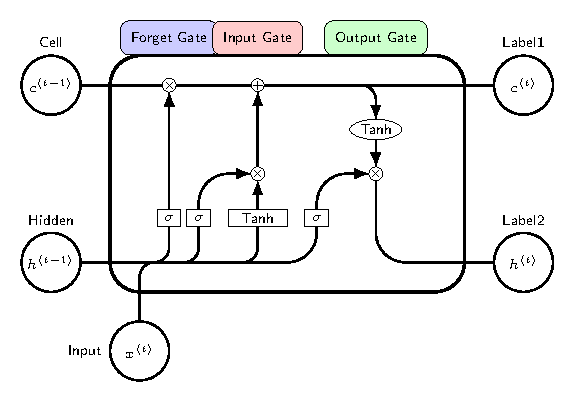
\includegraphics{draw_lstm.pdf}

}

\caption{\label{fig-lstm}Inner structure of a Long Short-Term Memory
Cell}

\end{figure}

This performance in modeling long-range dependencies has been validated
in various studies. The key component of LSTM's innovation is its memory
cell, \(c_t\)t, which stores state information, also refered to as
long-term memory. This cell is accessed, modified, and reset through
several self-parameterized gates. For the input of the sequence \(x_t\)
input, the forget gate \(f_t\) defines the percentage of the previous
long-term memory status \(c_{t-1}\) that should be retained
stored\hspace{0pt}. Next the input gate \(i_t\) decides how much of the
input is added to the the long-term memory, forming the updated cell
state \(c_{t}\). The decision to propagate the latest cell output,
\(c_t\), to the final state, \(h_t\), is governed by the output gate,
\(o_t\), representing the updated short-term memory of the hidden state
\(h_t\). A significant advantage of this architecture is the memory
cell's ability to retain gradients. This mechanism addresses the
vanishing gradient problem, where, as input sequences elongate, the
influence of initial stages becomes harder to capture, causing gradients
of early input points to approach zero. The LSTM's activation function,
inherently recurrent, mirrors the identity function with a consistent
derivative of 1.0, ensuring the gradient remains stable throughout
backpropagation.

One LSTM cell hence maybe expressed as:

\[
\begin{aligned}
i_t &= \sigma(W_{xi} x_t + W_{hi} h_{t-1} + W_{ci} \circ c_{t-1} + b_i) \\
f_t &= \sigma(W_{xf} x_t + W_{hf} h_{t-1} + W_{cf} \circ c_{t-1} + b_f) \\
c_t &= f_t \circ c_{t-1} + i_t \circ \tanh(W_{xc} x_t + W_{hc} h_{t-1} + b_c) \\
o_t &= \sigma(W_{xo} x_t + W_{ho} h_{t-1} + W_{co} \circ c_t + b_o) \\
h_t &= o_t \circ \tanh(c_t)
\end{aligned}
\]

with

\begin{itemize}
\tightlist
\item
  \(x_t\): Input vector at time step \(t\).
\item
  \(h_{t-1}\): Hidden state from the previous time step.
\item
  \(C_{t-1}\): Cell state from the previous time step.
\item
  \(W\) and \(b\): Weight matrices and bias vectors, respectively,
  associated with the gates of the LSTM. The subscripts denote the
  specific gate or operation they are associated with (e.g., \(W_f\) and
  \(b_f\) are the weight matrix and bias for the forget gate,
  respectively).
\item
  \(\sigma\): Sigmoid activation function, which squashes values between
  0 and 1.
\item
  \(\tanh\): Hyperbolic tangent activation function, which squashes
  values between -1 and 1
\end{itemize}

\hypertarget{convlstm-network}{%
\subsubsection{ConvLSTM network}\label{convlstm-network}}

The FC-LSTM fails to handle information when handling spatiotemporal
data due to its reliance on full connections in both input-to-state and
state-to-state transitions. To adress this limitation we use a convLSTM
architecture. convLSTM replaces the fully connected operations in the
LSTM with convolutional operations. Hence, all inputs
\(X_1, \ldots, X_t\), cell outputs \(C_1, \ldots, C_t\), hidden states
\(H_1, \ldots, H_t\), and gates \(i_t, f_t, o_t\) of the ConvLSTM are 3D
tensors. The last two dimensions of these tensors represent spatial
dimensions, specifically rows and columns. Conceptually, these inputs
and states can be visualized as vectors positioned on a spatial grid.

In the ConvLSTM, the future state of a specific cell on this grid is
determined by the inputs and past states of its neighboring cells. This
spatial consideration is integrated by employing a convolution operator
in both state-to-state and input-to-state transitions, as illustrated in
Fig. 2. The foundational equations for ConvLSTM are:

\[
\begin{aligned}
i_t &= \sigma(W_{xi} \ast X_t + W_{hi} \ast H_{t-1} + W_{ci} \circ C_{t-1} + b_i) \\
f_t &= \sigma(W_{xf} \ast X_t + W_{hf} \ast H_{t-1} + W_{cf} \circ C_{t-1} + b_f) \\
C_t &= f_t \circ C_{t-1} + i_t \circ \tanh(W_{xc} \ast X_t + W_{hc} \ast H_{t-1} + b_c) \\
o_t &= \sigma(W_{xo} \ast X_t + W_{ho} \ast H_{t-1} + W_{co} \circ C_t + b_o) \\
H_t &= o_t \circ \tanh(C_t)
\end{aligned}
\]

In summary, the ConvLSTM excels at processing tasks that demand a
combined understanding of spatial patterns and temporal sequences in
data. It merges the image-processing capabilities of Convolutional
Neural Networks (CNNs) with the time-series modeling of Long Short-Term
Memory (LSTM) networks.

\hypertarget{implemented-model-architecture}{%
\subsubsection{Implemented model
architecture}\label{implemented-model-architecture}}

We first implemented the ConvLSTM using and encoder/decoder structure as
discussed in \ldots{} . To predict all 97 rivers entering the Baltic Sea
at once, we flatten the output and use fully connected layers resulting
in 97 outputs.

For the computation we use the following set of hyper parameters:

\hypertarget{tbl-letters}{}
\begin{longtable}[]{@{}ll@{}}
\caption{\label{tbl-letters}Hyperparameters}\tabularnewline
\toprule()
Parameter name & Parameter size \\
\midrule()
\endfirsthead
\toprule()
Parameter name & Parameter size \\
\midrule()
\endhead
Num. timesteps & 32 \\
Conv. Kernelsize & (7,7) \\
Num. ConvLSTM layers & 4 \\
Batch size & 32 \\
~Learning Rate & 1e-4 with CosineAnnealing \\
\bottomrule()
\end{longtable}

\hypertarget{acknowledgments}{%
\subsection{Acknowledgments}\label{acknowledgments}}

Phasellus interdum tincidunt ex, a euismod massa pulvinar at. Ut
fringilla ut nisi nec volutpat. Morbi imperdiet congue tincidunt.
Vivamus eget rutrum purus. Etiam et pretium justo. Donec et egestas sem.
Donec molestie ex sit amet viverra egestas. Nullam justo nulla,
fringilla at iaculis in, posuere non mauris. Ut eget imperdiet elit.

\hypertarget{open-research}{%
\subsection{Open research}\label{open-research}}

Phasellus interdum tincidunt ex, a euismod massa pulvinar at. Ut
fringilla ut nisi nec volutpat. Morbi imperdiet congue tincidunt.
Vivamus eget rutrum purus. Etiam et pretium justo. Donec et egestas sem.
Donec molestie ex sit amet viverra egestas. Nullam justo nulla,
fringilla at iaculis in, posuere non mauris. Ut eget imperdiet elit.

\hypertarget{references}{%
\subsection*{References}\label{references}}
\addcontentsline{toc}{subsection}{References}

\hypertarget{refs}{}
\begin{CSLReferences}{0}{0}
\end{CSLReferences}



\end{document}
